\documentclass{ximera}

%\documentclass{ximera}

\usepackage{float}
\usepackage{subcaption}

\pgfplotsset{compat=1.16}

\newtheorem{ass}{Assumption}

\def\check{\tikz\fill[scale=0.4](0,.35) -- (.25,0) -- (1,.7) -- (.25,.15) -- cycle;}





\outcome{We will see some more advanced applications of the Black-Scholes formula. Gap options will be covered.}

\author{Brad Waller}

%Section 4.5

\title{Examples (Advanced)}

\begin{document}
\begin{abstract}
Previously, we saw some elementary applications of the Black-Scholes formula. Here, we will see some more advanced applications. This includes the more general Black-Scholes formula.
\end{abstract}
\maketitle

We have seen several examples of the Black-Scholes formula in action. This section deals with some consequences of that formula, and it covers some new concepts that result from using the formula. Let's begin with what was promised: the proof of put-call duality. Recall the formulae for duality:

\begin{align*}
c(S,K) 	&=S\cdot K\cdot p(1/S,1/K)\\
p(S,K)		&=S\cdot K\cdot c(1/S, 1/K)
\end{align*}

We will prove that the first formula holds and leave the second to the reader. To prove it, we just apply the Black-Scholes formula to each side. We begin with the left-hand side. $\delta$ will represent the risk-free rate for the asset currency in this part.

\begin{align*}
d_1 		&=\frac{\ln\frac{S(0)}{K}+(r-\delta+\sigma^2/2)T}{\sigma\sqrt{T}}\\
d_2 		&=\frac{\ln\frac{S(0)}{K}+(r-\delta-\sigma^2/2)T}{\sigma\sqrt{T}}\\
c 		&=S(0)e^{-\delta T}\mathcal{N}(d_1)-Ke^{-rT}\mathcal{N}(d_2)
\end{align*}

Now, we apply the formula to the right hand side. Due to the ambiguity in using $d_1$ and $d_2$ again, we will use tildes over the d's. Recall that the asset for the right hand side is $1/S$ and the strike is $1/K$. In the computations here, the roles of $\delta$ and $r$ are reversed. Finally, the volatility remaines unchanged since it is the same measurement between these two assets. If you aren't convinced of this part, just reverse the order of your fractions from a volatility computation. The sample variance will remain unchanged.

\begin{align*}
\tilde{d}_1 				&=\frac{\ln\frac{1/S(0)}{1/K}+(\delta-r+\sigma^2/2)T}{\sigma\sqrt{T}}\\
					&=-\frac{\ln\frac{S(0)}{K}+(r-\delta-\sigma^2/2)T}{\sigma\sqrt{T}}\\
					&=-d_2\\
\tilde{d}_2 				&=\frac{\ln\frac{1/S(0)}{1/K}+(\delta-r-\sigma^2/2)T}{\sigma\sqrt{T}}\\
					&=-\frac{\ln\frac{S(0)}{K}+(r-\delta+\sigma^2/2)T}{\sigma\sqrt{T}}\\
					&=-d_1
\end{align*}

That's rather convenient! Let's put these values into the Black-Scholes formula for the put option.

\begin{align*}
p 					&=1/Ke^{-\delta T}\mathcal{N}(-d_2)-1/S(0)e^{-rT}\mathcal{N}(-d_1)\\
					&=1/Ke^{-\delta T}\mathcal{N}(d_1)-1/S(0)e^{-rT}\mathcal{N}(d_2)\\
S(0)\cdot K\cdot p(1/S,1/K) 	&=S(0)e^{-\delta T}\mathcal{N}(d_1)-Ke^{-rT}\mathcal{N}(d_2)\\
					&=c(S,K)
\end{align*}

It's good that we could validate the formula we came up with some time ago. If you want an extra challenge, try to verify the formula using a binomial model. I've never tried it myself, but it would be a fun exercise. My suspicion is that it will work for the Cox-Ross-Rubenstein and the Forward tree models. You may run into some difficulty with the Jarrow-Rudd model.

Let's move our attention on to the subject of gap options. A gap option is simply a modified call or put option. 

\begin{definition}
A {\bf gap option} is an option with strike $K_1$ and payoff equal to 
	\begin{equation*}
	\max\{S(t)-K_2,0\}
	\end{equation*}
for a gap call and payoff equal to 
	\begin{equation*}
	\max\{K_2-S(t),0\}
	\end{equation*}
for a gap put. The payoffs are at time $t$.
\end{definition}

The given definition allows for American gap options; however, we will only consider the case when they are European. That is, we will price them with an expiration time of $T$. Before we work out some prices, it is useful to visualize these options. 

\begin{center}
	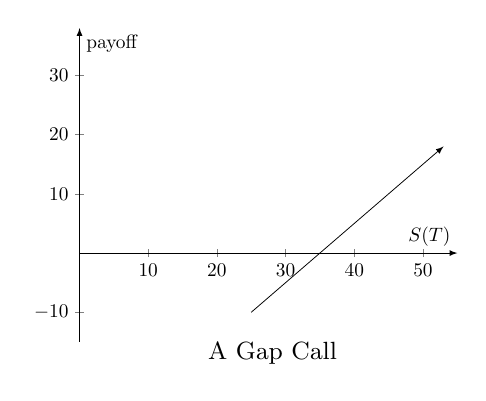
\begin{tikzpicture}[scale=0.7]
	\begin{axis}[
		xmin=0,
		xmax=55,
		%xtick={5,10,...,50},
		ymin=-15,
		ymax=38,
		%ytick={-20,-10,...,50},
		%grid=both,
		axis lines=middle,
		axis line style={->, >=latex},
		%x label style={at={(0.9,0.05)}},
		%x label style={at={(axis description cs:0.86,0.42)},anchor=north},
		xlabel={$S(T)$},
		ylabel={payoff}]
		%style={font=\tiny}]
		\addplot[black, smooth, domain=25:53, ->, >=latex]{x-35};
	\end{axis}
	\node at (3.5, -0.2) {\small A Gap Call};
	\end{tikzpicture}
	\hspace{10pt}
	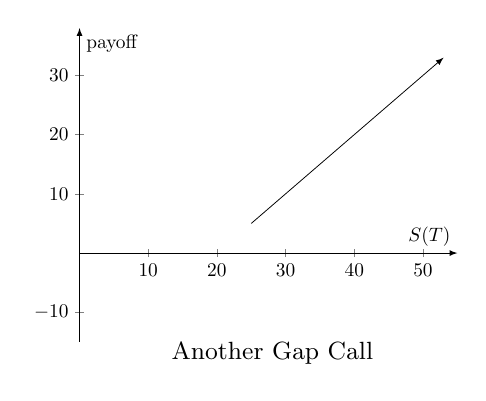
\begin{tikzpicture}[scale=0.7]
	\begin{axis}[
		xmin=0,
		xmax=55,
		%xtick={5,10,...,50},
		ymin=-15,
		ymax=38,
		%ytick={-20,-10,...,50},
		%grid=both,
		axis lines=middle,
		axis line style={->, >=latex},
		%x label style={at={(axis description cs:0.86,0.42)},anchor=north},
		xlabel={$S(T)$},
		ylabel={payoff}]
		%style={font=\tiny}]
		\addplot[black, smooth, domain=25:53, ->, >=latex]{x-20};
	\end{axis}
	\node at (3.5, -0.2) {\small Another Gap Call};
	\end{tikzpicture}
\end{center}

Both of the options in the figure can be viewed as gap options, but it is more useful if you can view them as combinations of asset-or-nothing options combined with cash-or-nothing options where each option has the same strike, $K=25$. The first gap call should have a price equivalent to a strike 25 asset-or-nothing option with 35 written cash-or-nothing options. The second gap call should have a price equivalent to a strike 25 asset-or-nothing options with 20 written cash-or-nothing options. When this is written, it would look like this:

\begin{align*}
c_{\text{gap},1} 	&=S(0)e^{-\delta T}\mathcal{N}(d_1)-35e^{-rT}\mathcal{N}(d_2)\\
c_{\text{gap},2} 	&=S(0)e^{-\delta T}\mathcal{N}(d_1)-20e^{-rT}\mathcal{N}(d_2)
\end{align*}

Do not make the mistake and assume that $K=35$ or $K=20$ in your computations of $d_1$ and $d_2$! That is a pitfall that many stumble into. In both, the values for $d_1$ and $d_2$ are identical.

\begin{align*}
d_1 	&=\frac{\ln\frac{S(0)}{25}+(r-\delta+\sigma^2/2)T}{\sigma\sqrt{T}}\\
d_2 	&=\frac{\ln\frac{S(0)}{25}+(r-\delta-\sigma^2/2)T}{\sigma\sqrt{T}}
\end{align*}

To complete our visualization, let's graph the gap puts as well.

\begin{center}
	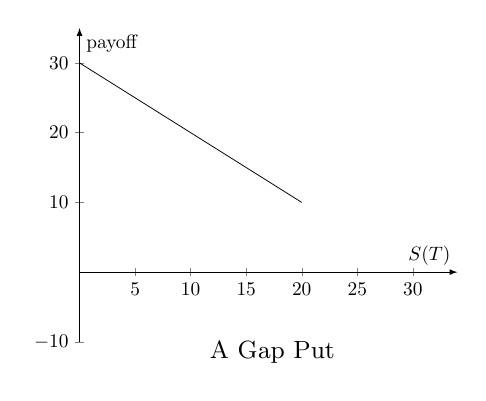
\begin{tikzpicture}[scale=0.7]
	\begin{axis}[
		xmin=0,
		xmax=34,
		%xtick={5,10,...,50},
		ymin=-10,
		ymax=35,
		%ytick={-20,-10,...,50},
		%grid=both,
		axis lines=middle,
		axis line style={->, >=latex},
		%x label style={at={(0.9,0.05)}},
		%x label style={at={(axis description cs:0.86,0.42)},anchor=north},
		xlabel={$S(T)$},
		ylabel={payoff}]
		%style={font=\tiny}]
		\addplot[black, smooth, domain=0:20, -, >=latex]{30-x};
	\end{axis}
	\node at (3.5, -0.2) {\small A Gap Put};
	\end{tikzpicture}
	\hspace{10pt}
	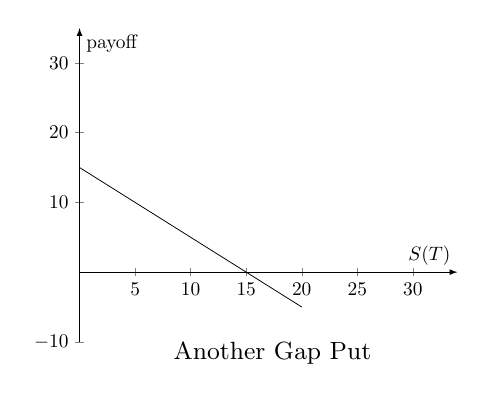
\begin{tikzpicture}[scale=0.7]
	\begin{axis}[
		xmin=0,
		xmax=34,
		%xtick={5,10,...,50},
		ymin=-10,
		ymax=35,
		%ytick={-20,-10,...,50},
		%grid=both,
		axis lines=middle,
		axis line style={->, >=latex},
		%x label style={at={(axis description cs:0.86,0.42)},anchor=north},
		xlabel={$S(T)$},
		ylabel={payoff}]
		%style={font=\tiny}]
		\addplot[black, smooth, domain=0:20, -, >=latex]{15-x};
	\end{axis}
	\node at (3.5, -0.2) {\small Another Gap Put};
	\end{tikzpicture}
\end{center}

Both of the put options have the same strike, $K=20$. To get the first gap put, you could purchase an asset-or-nothing put and buy 10 cash-or-nothing puts. The get the second gap put, you could purchase an asset-or-nothing put and write 5 cash-or-nothing puts.

We can summarize what we have done in the following theorem.

\begin{theorem}[Gap Options]
The Black-Scholes price for gap calls and gap puts are given by the formulae below.
	\begin{align*}
	c_{\text{gap}} 	&=S(0)e^{-\delta T}\mathcal{N}(d_1)-K_2e^{-rT}\mathcal{N}(d_2)\\
	p_{\text{gap}} 	&=K_2e^{-rT}\mathcal{N}(-d_2)-S(0)e^{-\delta T}\mathcal{N}(-d_1)\\
	d_1 			&=\frac{\ln\frac{S(0)}{K_1}+(r-\delta+\sigma^2/2)T}{\sigma\sqrt{T}}\\
	d_2			&=\frac{\ln\frac{S(0)}{K_1}+(r-\delta-\sigma^2/2)T}{\sigma\sqrt{T}}
	\end{align*}
\end{theorem}

\begin{question}
You wish to purchase a European gap option on an asset, $S$. The option pays
	\begin{equation*}
		\begin{cases}
		S(1/3)-40	 &\text{if }S(1/3)>35,\\
		0 		&\text{otherwise}
		\end{cases}
	\end{equation*}
in four months. Determine the price of the option if
	\begin{itemize}
	\item $S(0)=37$\\
	\item $r=0.08$\\
	\item $\delta=0.02$\\
	\item $\sigma=0.34$
	\end{itemize}
The price is $\answer{1.32}$.
\end{question}

\begin{solution}
The answer must be of the form
	\begin{equation*}
	c_{\text{gap}}=37e^{-0.02/3}\mathcal{N}(d_1)-40e^{-0.08/3}\mathcal{N}(d_2),
	\end{equation*}
where $d_1$ and $d_2$ are given below.
	\begin{align*}
	d_1 			&=\frac{\ln\frac{37}{35}+(0.08-0.02+0.34^2/2)/3}{0.34\sqrt{1/3}}\\
				&=0.483\\
	d_2 			&=d_1-0.34\cdot\sqrt{1/3}\\
				&=0.287\\
	c_{\text{gap}} 	&=37e^{-0.02/3}\mathcal{N}(0.483)-40e^{-0.08/3}\mathcal{N}(0.287)\\
				&=36.75\cdot 0.68545-38.95\cdot 0.61294\\
				&=1.32
	\end{align*}
\end{solution}

As you likely noticed, the hardest part when dealing with gap options is the appearance that there are two strikes. I keep this straight in my head by remembering that the payoff is immediately clear from the Black-Scholes formula that you write down. The was that is displayed above is

\begin{align*}
S(1/3)-&40\\
S(1/3)e^{-\delta/3}\mathcal{N}(d_1)-&40e^{-r/3}\mathcal{N}(d_2).
\end{align*}

The $40$ appears in the payoff and the price. That leaves the value from the ``if`` statement for the computations of $d_1$ and $d_2$. 

We conclude this section with the notion of implied volatility. As you may have noticed, there are aobut six variables that go into every Black-Scholes formula computation: $S$, $K$, $r$, $\delta$, $\sigma$ and $T$. In almost all situations you encounter, five of those variables will be public information. That is, all the variables except volatility are known. An argument can be made regarding the risk-free rate and the dividend rate; however, those remain constant in the short term for almost all situations. $S$, $K$, and $T$ are all defined in a contract.

What all this means is that if we encounter an option price, then we can deduce the volatility under the Black-Scholes model from that price. This sounds a little daunting since the formula relies on some normal table values. The reality is not so terrible. If you want to use technology, program the Black-Scholes formula into Excel. Then you can use Excel's goal seek feature to determine the volatility given the other five constants from the Black-Schole formula. For example, I used the values from the previous problem. I decided that the price of some call option under similar conditions was 5. This gave me an implied volatility of 0.43.

Obviously, this is not how this kind of question would appear on an exam or homework assignment. You would need to use some sort of algebraic manipulations to back out the appropriate result. Let's see how one might do that in an example.

\begin{example}
You observe the price of a six month, strike 59  European call is $7.64$. The current underlying asset's price is $57$, the dividend rate is $0.01$, and the risk-free rate is $0.079$. Determine the implied volatility.
\end{example}

\begin{solution}
We use the Black-Scholes formula. First, we solve for $d_1$ and $d_2$ and hope for the best.
	\begin{align*}
	d_1 			&=\frac{\ln{57}{59}+(0.079-0.01+\sigma^2/2)/2}{\sigma\sqrt{1/2}}\\
				&=\frac{(\sigma^2/2)/2}{\sigma\sqrt{1/2}}\\
				&=\sigma\cdot\frac{\sqrt{2}}{4}\\
	d_2			&=d_1-\sigma\sqrt{1/2}\\
				&=-\sigma\cdot\frac{\sqrt{2}}{4}\\
				&=-d_1\\
	c 			&=7.64\\
				&=57e^{-0.01/2}\mathcal{N}(d_1)-59e^{-0.079/2}\mathcal{N}(-d_1)\\
				&=57e^{-0.01/2}[\mathcal{N}(d_1)-\mathcal{N}(-d_1)]\\
				&=57e^{-0.01/2}[2\mathcal{N}(d_1)-1]
	\end{align*}

The last two steps require some justification. In the first, $57e^{-0.01/2}$ is factored out of the equation. That is because the value $59$ is the forward price of the asset. Once we discount that value at the risk-free rate we have $S(0)e^{-0.01/2}$, the prepaid forward price. The last step follows by the symmetry of the standard normal distribution. $\mathcal{N}(-d_1)$ represents the left tail value that is equivalent to the probability $\mathbb{P}(\mathcal{N}(0,1)>d_1)=1-\mathbb{P}(\mathcal{N}(0,1)<d_1)$. 

Now we just unravel $d_1$ from the equations we wrote above. 

	\begin{align*}
	7.64 		&=57e^{-0.01/2}[2\mathcal{N}(d_1)-1]\\
	7.64/56.71 	&=[2\mathcal{N}(d_1)-1]\\
	1.13471 	&=2\mathcal{N}(d_1)\\
	0.56736 	&=\mathcal{N}(d_1)\\
	0.16966	&=d_1
	\end{align*}

Now we have a formula for $\sigma$!

	\begin{align*}
	0.16966 	&=\sigma\cdot \frac{\sqrt{2}}{4}\\
	0.47987 	&=\sigma	
	\end{align*}

\end{solution}

I actually used $\sigma=0.48$ in my original formula for the price of this particular option. Any of the steps could have picked up a slight rounding error, but I think $0.47987$ is probably good enough!

That concludes our topics that apply the Black-Scholes model in a direct way. Our next section will cover another Black-Scholes formula topic where you buy some asset using an asset (other than cash). This seems more like a barter, but the formula that describes the activity turns out to be identical to the Black-Scholes formula. 

\end{document}
